\documentclass[a4paper,10pt]{article}
\usepackage[margin=2.5cm]{geometry}

\usepackage{amssymb,amsmath,amsthm}
\usepackage{color}
\usepackage{enumitem}
\usepackage{dsfont}
\usepackage{bm}


\newtheorem{theorem}{Theorem}
\newtheorem{proposition}{Proposition}
\newtheorem{cor}{Corollary}
\theoremstyle{definition}
\newtheorem{definition}{Definition}
\newtheorem{remark}{Remark}
\newtheorem{example}{Example}
\newtheorem{claim}{Claim}
\newtheorem{lemma}{Lemma}


%%%%%%%%%%%%%%%%%%%%%%%%%%%%%%%%%%%%%%%%%%%%%%%%%%%%%%%%%%%%%%%%%%%%%%%%%%%%%%%
% Algorithms
%%%%%%%%%%%%%%%%%%%%%%%%%%%%%%%%%%%%%%%%%%%%%%%%%%%%%%%%%%%%%%%%%%%%%%%%%%%%%%%

\usepackage{algorithm}
\usepackage{algorithmic}
\usepackage[titlenumbered,ruled,noend,algo2e]{algorithm2e}
\newcommand\mycommfont[1]{\footnotesize\ttfamily\textcolor{blue}{#1}}
\SetCommentSty{mycommfont}
\SetEndCharOfAlgoLine{}


%%%%%%%%%%%%%%%%%%%%%%%%%%%%%%%%%%%%%%%%%%%%%%%%%%%%%%%%%%%%%%%%%%%%%%%%%%%%%%%
% Code
%%%%%%%%%%%%%%%%%%%%%%%%%%%%%%%%%%%%%%%%%%%%%%%%%%%%%%%%%%%%%%%%%%%%%%%%%%%%%%%


\usepackage{fancyvrb}                  % for fancy verbatim
\usepackage{textcomp}
\usepackage[space=true]{accsupp}
% requires the latest version of package accsupp
\newcommand{\copyablespace}{
    \BeginAccSupp{method=hex,unicode,ActualText=00A0}
\ %
    \EndAccSupp{}
}
\usepackage[procnames]{listings}
% \usepackage{setspace} % need for \setstretch{1}
\lstset{%
language   = python,%
 % basicstyle = \ttfamily\setstretch{1},%
basicstyle = \ttfamily,%
columns    = flexible,%
keywordstyle=\color{javared},
firstnumber=100,
frame=shadowbox,
showstringspaces=false,
morekeywords={import,from,class,def,for,while,if,is,in,elif,
else,not,and,or,print,break,continue,return,True,False,None,access,
as,del,except,exec,finally,global,import,lambda,pass,print,raise,try,assert,!=},
keywordstyle={\color{javared}\bfseries},
commentstyle=\color{javagreen}, %vsomb_col white comments
morecomment=[s][\color{javagreen}]{"""}{"""},
upquote=true,
%% style for number
numbers=none,
resetmargins=true,
xleftmargin=10pt,
linewidth= \linewidth,
numberstyle=\tiny,
stepnumber=1,
numbersep=8pt, %
frame=shadowbox,
rulesepcolor=\color{black},
procnamekeys={def,class},
procnamestyle=\color{oneblue}\textbf,
literate={á}{{\'a}}1
{à}{{\`a }}1
{ã}{{\~a}}1
{é}{{\'e}}1
{ê}{{\^e}}1
{è}{{\`e}}1
{í}{{\'i}}1
{î}{{\^i}}1
{ó}{{\'o}}1
{õ}{{\~o}}1
{ô}{{\^o}}1
{ú}{{\'u}}1
{ü}{{\"u}}1
{ç}{{\c{c}}}1
}


\usepackage{times} % use Times

\usepackage{../sty/shortcuts_js} % possibly adapted from https://github.com/josephsalmon/OrganizationFiles/sty/shortcuts_js.sty

%%%%%%%%%%%%%%%%%%%%%%%%%%%%%%%%%%%%%%%%%%%%%%%%%%%%%%%%%%%%%%%%%%%%%%%%%%%%%%%
% IMAGES
%%%%%%%%%%%%%%%%%%%%%%%%%%%%%%%%%%%%%%%%%%%%%%%%%%%%%%%%%%%%%%%%%%%%%%%%%%%%%%%

% Use prebuiltimages/ for images extracted from code (e.g. python)
% or to share images built from a software not available by the whole team (say matlab .fig, or inskcape .svg).
% .svg files should be stored in dir srcimages/ and built from moosetex if needed:
% https://www.charles-deledalle.fr/pages/moosetex.php
% NEVER (GIT) versions files in images/ : only prebuiltimages/ & srcimages/ !

\usepackage{graphicx} % For figures
\graphicspath{{images/}, {prebuiltimages/}}
\usepackage{subcaption}


%%%%%%%%%%%%%%%%%%%%%%%%%%%%%%%%%%%%%%%%%%%%%%%%%%%%%%%%%%%%%%%%%%%%%%%%%%%%%%%
% For citations
%%%%%%%%%%%%%%%%%%%%%%%%%%%%%%%%%%%%%%%%%%%%%%%%%%%%%%%%%%%%%%%%%%%%%%%%%%%%%%%

\usepackage[authoryear]{natbib}
\usepackage{cleveref} % mandatory for no pbs with hyperlinks theorem etc...
\crefformat{equation}{Eq.~(#2#1#3)} % format for equations
\Crefformat{equation}{Equation~(#2#1#3)} % format for equations


%%%%%%%%%%%%%%%%%%%%%%%%%%%%%%%%%%%%%%%%%%%%%%%%%%%%%%%%%%%%%%%%%%%%%%%%%%%%%%%
% Header and document start
%%%%%%%%%%%%%%%%%%%%%%%%%%%%%%%%%%%%%%%%%%%%%%%%%%%%%%%%%%%%%%%%%%%%%%%%%%%%%%%


\author{Rudolf Römisch}
\title{Noisy and Missing Data Regression: Distribution-Oblivious Support Recovery}

\begin{document}

\maketitle

\vskip 0.3in

\begin{abstract}
Many models for sparse regression typically assume that the covariates are known completely and without noise. Particularly in high-dimensional applications, this is often not the case. Worse yet, even estimating statistics of the noise (the noise covariance) can be a central challenge.  
We consider the development of a simple variant of orthogonal matching pursuit (OMP) for the setting described before. We show that without knowledge of the noise covariance, the algorithm recovers the support and we provide matching lower bounds that show that the algorithm performs at the minimax optimal rate. Noticably, this algorithm is the first that recovers support in a noise-distribution-oblivious manner. We even have for the case of knowledge of the noise-covariance matching between this algorithm and the best-known $l^2$-recovery bounds available. We also have that both are min-max optimal.
\end{abstract}

\section{Introduction}


This work considers the case of high-dimensionality. It is of special interest since standard algorithms have higher sensivity. Noisy data or even missing data can be costly for standard algortihms. In the worst case it can prevent a proper estimation and research of the statistics and noise of the model. \\
We study that case and give reasonable research and results with bounds and inequalities which happen to optimize the case. Maybe we even give a new standard way of estimating in linear regression with sparsity recovery and only partially known noise covariance.

\subsection{Main Results}
\begin{itemize}
	\item OMP and Support Recovery: We give conditions for when $standard$ $OMP$ guarantees exact support recovery in the missing and noisy covariate setting. Our results do not require knowledge of $\mathbb{E}[W^TW]$ (the noise covariance) or $\rho$ (the erasure probability). Other approaches require this knowledge, and our simulations indicate the dependence is real. 
	\item $l^2$-bounds: Even if the noise covariance is known, standard OMP does not provide competitive $l^2$-bounds. We design simple estimators based on either knowledge of the statistics of the covariate noise, ot the covariate distribution. We provide finite sample performance guarantees that are as far as we know, the best available. In the supplemental section, we show we can also obatin such bounds using in Instrumental Variable correlated with the covariates. We are not aware of any rigorous finite sample results in this setting.
	\item In simulations, the advantage of our algorithm seems more pronounced, in terms of both speed and statistical performance. Moreover, while we provide no analysis for the case of correlated columns of the covariate matrix, our simulations indicate that the impediment is in the analysis, as the results for our algorithm seem very promising.
	\item Finally, as a corollary to our results above, setting the covariate-noise-level to zero, we obtain bounds on the performance of OMP in the standard setting, with additive Gaussian noise. Our bounds are better than bounds obtained by specializing deterministic results and ignoring Gaussianity.
\end{itemize}

Another important mention is that OMP-like methods are signicantly easier to implement and computationally less
demanding. Therefore, particularly for large-scale
applications, understanding their performance is important,
and they have a role to play even where
optimization-based algorithms have proven successful.
In this case, we have both the simplicity of OMP and
the guarantee of distribution-oblivious recovery.



\newpage
\section{Problem Setup}
Now we describe the specific setting we operate. Therefore we need to introduce some notations and definitions.
We denote our unknown k-sparse regressor (or signal) in $\mathbb{R}^p$ as $\beta^*$. We obtain measurements $y_i\in \mathbb{R}$ according to the linear model
\begin{equation*}
	y_i = \langle x_i,\beta^*\rangle + e_i, \quad	i=1,...,n
\end{equation*}
Here, $x_i$ is a covariate vector of dimension p and $e_i \in \mathbb{R}$ is additive error. We are interested in the standard high-dimensional scaling, where $n=O(klog(p))$.\\
The standard setting assumes that each covariate vector $x_i$ is known directly, and exactly. Instead, here we assume we only observe a vector $z_i \in \mathbb{R}^p$ which is linked to $x_i$ via some distribution that may be unknown to the algorithm. We focus on two cases:\\
\begin{itemize}
	\item[1.] Covariates with additive noise: We observe $z_i=x_i+w_i$, where the entries of $w_i \in \mathbb{R}^p(or \mathbb{R}^k)$ are independent of each other and everything else.
	\item[2.] Covariates with missing data: We consider the case where the entries of $x_i$ are observed independently with probability $1-\rho$, and missing with propability $\rho$.
\end{itemize}
\ \\
We consider the case where the covariate matrix X, the covariate noise W and the additive noise vector e are sub-Gaussian. We give the basic definitions here, as these are used throughout.

\begin{definition}\ \\
	Sub-Gaussian Matrix: A zero-mean matrix V is called sub-Gaussian with parameter $(\frac{1}{n}\Sigma,\frac{1}{n}\sigma^2)$ if (a) Each row $v_i^T \in \mathbb{R}^p$ of V is sampled independently and has $\mathbb{E}[v_iv_i^T]=\frac{1}{n}\Sigma$. (b) For any unit vector $u \in \mathbb{R}^p$, $u^Tv_i$ is a sub-Gaussian random variable with parameter at most $\frac{1}{\sqrt{n}}\sigma$.
\end{definition}

\begin{definition}\ \\
	Sub-Gaussian Design Model: We assume X, W and e are sub-Gaussian with parameters $(\frac{1}{n}\Sigma_x,\frac{1}{n})$, $(\frac{1}{n}\Sigma_w, \frac{1}{n}\sigma_w)$ and $(\frac{1}{n}\sigma_e^2, \frac{1}{n}\sigma_e^2)$, respectively, and are independent of each other. For the case of independence across columns we call this the $Independent$ sub-Gaussian Model.
\end{definition}

\section{Distribution-Oblivious Support Recovery via Orthogonal Matching Pursuit}
In the case of additive noise, both the modified Dantzig selector and the modified Lasso can be viewed as trying to find the $l^1$ constrained solution that satisfies the first order condition $(Z^TZ - \Sigma_w)\beta-Z^Ty \approx 0$. Knowing $\Sigma_w$ is necessary in order to construct the matrix $Z^TZ-\Sigma_w$, which is an unbiased estimator of $\Sigma_x$; otherwise, solving the uncompensated condition $Z^TZ\beta - Z^Ty ~ 0$ will consistently underestimate $\beta^*$ even in the low-dimensional case. This seems unavoidable if the goal is to estimate the values of $\beta^*$.

\subsection{Support Identification}
Given a matrix Y and index set I, we use $Y_I$ to denote the sub matrix with columns of Y indexed by I. We consider the following OMP algorithm, given in Algorithm 1. We call this supp-OMP to emphasize that its output is the support set, not $\hat{\beta}$. At each iteration, it computes the inner product between $Z_i$ and the $residual$ $r_t$ instead of the original y, and picks the index with largest magnitude.\\
We give some intuition on why one should expect supp-OMP would work without knowing $\Sigma_w$. Let $I_t$ be the set of columns selected in the first t iterations of OMP; we assume the first t iterations succeed so $I_t \subset I^*$. Observe that OMP succeeds as long as the following two conditions are satisfied:
\begin{itemize}
	\item $\langle Z_i,r_t\rangle = 0$, for all $i\in I_t$.
	\item $\langle Z_i,r_t\rangle > \langle Z_j,r_t\rangle$, for all $i \in I^*/I_t$ and $j\in (I^*)^c$.
\end{itemize}

The first condition is satisfied automatically, due to the way we compute the residual $r_t = (I-\mathcal{P})y \equiv (I-Z_{I_t}(Z_{I_t}^TZ_{I_t})^{-1}Z_{I_t}^T)y;$ in particular, we orthogonalize y against $Z_{I_t}$, not $X_{I_t}$. Now consider the second condition. Observe that, for each $i\in I^c_t$, we have
\begin{equation*}
	\langle Z_i, r_t \rangle = \langle Z_i,y \rangle - \langle Z_i, \mathcal{P}_ty \rangle = \langle Z_i,y \rangle - Z_i^T Z_{I_t} \tilde{\beta}_t
\end{equation*}
where $\tilde{\beta}_t = (Z_{I_t}^T Z_{I_t})^{-1}Z_{I_t}^Ty.$ We call this $\tilde{\beta}$ because it is not the best estimate one could obtain, if the noise covariance were known. Indeed, there is an $\mathbb{E}[W^TW]$ term embedded inside $\tilde{\beta}$, which, as discussed, is an underestimate of $\beta^*$ as it is produced without compensating for the effect of $W^TW$. The key insight and idea of the proof, is to show that despite the presence of this error, the dominating term is unbiased, so the ordering of the inner products is unaffected.

The next theorem gives the performance of supp-OMP for distribution-oblivious support recovery.

\begin{theorem}\ \\
	Under the Independent sub-Gaussian Design model and Additive Noise model, supp-OMP identifies the correct support of $\beta^*$ with high probability, provided
	\begin{equation*}
		n \gtrsim (1+\sigma^2_w)^2klog(p),
	\end{equation*}
	\begin{equation*}
		|\beta^*_i| \geq 16(\sigma_w||\beta^*||_2 + \sigma_e)\sqrt{\frac{log(p)}{n}},
	\end{equation*}
	for all $i \in supp(\beta^*)$.
\end{theorem}
One notices two features of this result. Setting $\sigma_w = 0$ in Theorem 1, we obtain result that seem to better than previous probabilistic guarantees for OMP with Gaussian noise and clean covariates.



\begin{theorem}\ \\
	Let $\sigma^2_z = \sigma^2_x + \sigma^2_w$. Under the independent Gaussian model where the covariance of X, W and e are isotropic, if 
	\begin{align*}
		n &\lesssim (\sigma^2_w + \frac{\sigma^2_z \sigma^2_e}{R^2})k log(\frac{p}{k}) \quad or\\
		b_{min} &\lesssim \sqrt{(\sigma^2_w R^2 + \sigma^2_z \sigma^2_e) \frac{log(p/k)}{n}}, \quad then\\
		\mathcal{M}_0 &\geq 1.
	\end{align*}
\end{theorem}
Note the dependence on $R = ||\beta^*||_2$.

\subsection{Estimating the Non-Zero Coefficients}
Once the support of $\beta^*$ is identified, estimating its non-zero values $\beta^*_I$ becomes a low-dimensional problem. Given the output I of supp-OMP, we consider the following generic estimator
\begin{align}
	\hat{\beta}_I =& \hat{\Sigma}^{-1}\hat{\gamma},\\
	\hat{\beta}_{I^c} =& 0.
\end{align}

The estimator requires computing two matrices, $\hat{\Sigma}$ and $\hat{\gamma}$. If X is known, setting $\hat{\Sigma} = X^T_I X_I$ and $\hat{\gamma} = X^T_Iy$ gives the standard least squares estimator. For our problem where only Z is observed, some knowledge of X or the nature of the corruption (W in the case of additive noise) is required in order to proceed. For the case of additive noise, we consider two models for a priori knowledge of X or of the noise:
\begin{itemize}
	\item Knowledge of $\Sigma_w$: in this case, we assume we either know or somehow can estimate the noise covariance on the true support, $\Sigma^{(I)}_w = \mathbb{E}[W^T_IW_I]$. We then use $\hat{\Sigma} = Z^T_I Z_I - \Sigma^{(I)}_w$ and $\hat{\gamma} = Z^T_Iy$.
	\item Knowledge of $\Sigma_x$: we assume that we either know or somehow can estimate the covariance of the true covariates on the true support, $\Sigma^{(I)}_x = \mathbb{E}[X^T_I X_I]$. We then use $\hat{\Sigma} = \Sigma^{(I)}_x$ and $\hat{\Sigma} = Z^T_Iy$.
	\item Knowledge of $\rho$. we compute $\hat{\Sigma} = (Z^T_I Z_I) \odot M$ and $\hat{\gamma} = \frac{1}{(1-\rho)}Z^T_Iy$, where $M \in \mathbb{R}^{|I|\times|I|}$ satisfies $M_{ij} = \frac{1}{1-\rho}$ if $i=j$ or $\frac{1}{(1-\rho)^2}$ otherwise, and $\odot$ denotes element-wise product.
\end{itemize}

\begin{theorem}\ \\
	Under the Independent sub-Gaussian Design model and Additive Noise model, the output of estimator (2) satisfies:
	\begin{itemize}
		\item (Knowledge of $\Sigma_w$): $||\hat{\beta} - \beta^*||_2 \lesssim [(\sigma_w + \sigma_w^2)||\beta^*||_2 + \sigma_e \sqrt{1+\sigma_w^2}]\sqrt{\frac{klog(p)}{n}}$.
		\item (Knowledge of $\Sigma_x$): $||\hat{\beta} - \beta^*||_2 \lesssim [(1 + \sigma_w)||\beta^*||_2 + \sigma_e \sqrt{1+\sigma_w^2}]\sqrt{\frac{klog(p)}{n}}$.
	\end{itemize}
\end{theorem}

\begin{theorem}\ \\
	Let $\sigma_z^2 = \sigma_x^2 + \sigma_w^2$, and suppose $8 \geq k \geq p/2$ and $n \lesssim k log (p/k)$. Under the independent Gaussian model where the covariance of X, W and e are isotropic, the $l^2$-error is bounded below: $M_2 \gtrsim \sqrt{(\sigma_w^2 R^2 + \sigma_z^2 \sigma_e^2)\frac{k}{n} log(\frac{p}{k})}$.
\end{theorem}

\subsection{Missing Data}

The following theorem gives an analogous guarantee to theorem 1.

\begin{theorem}\ \\
	Under the Independent sub-Gaussian Design model and missing data model, supp-OMP identifies the correct support of $\beta^*$ provided
	\begin{align*}
		n &\gtrsim \frac{1}{(1-\rho)^4}k log(p),\\
		|\beta^*_i| &\geq \frac{16}{1-\rho}(||\beta^*||_2 + \sigma_e) \sqrt{\frac{log(p)}{n}},
	\end{align*}
	for all $i \in supp(\beta^*)$. Moreover; the output of estimator (2) with knowledge of $\rho$ satisfies
	\begin{equation*}
		||\hat{\beta} - \beta^*||_2 \lesssim (\frac{1}{(1-\rho)^2}||\beta^*||_2 + \frac{1}{1-\rho}\sigma_e)\sqrt{\frac{k log(p)}{n}}.
	\end{equation*}
\end{theorem}

Note that the condition on $|\beta_i|$ as well as the bounds for the $l^2$ error again depend on $||\beta^*||_2$, corresponding to a natural and necessary SNR requirement analogous to that in theorem 1. For $l^2$ error, our conditions and bound match those in previous work.



\section{Numerical Simulations}

The numerical results illustrate two main points. First, we show that the quality of support recovery using either the improved MU selector or the projected gradient algorithm based on modified Lasso, deteriorates significantly when $\Sigma_w$ is not known accurately. That is, if those algorithms use either upper or lower bounds on $\Sigma_w$ instead of the correct value. Throughout the range of comparison, our supp-OMP algorithm is unaffected by the inaccuracy of $\Sigma_w$ and recovers the support.

\subsection{Additive Noise}
For the additive noise case, we use the following setting:\\
$p=450, n=400, \sigma_e=0, \Sigma_x = I,k\in \{2,...,7\}$, and $\sigma_w \in [0,1]$.\\
The data X, W and e are generated from (isotropic) Gaussian distribution. We first consider support recovery and study the robustness of the three methods to over- or under-estimating $\Sigma$. For low noise, the performance is largely unaffected. It quickly deteriorates as the noise level grows. The graph below shows this deterioration.\\
(a) show results when $\Sigma_w = \Sigma^{true}_w/ 2$ and (b) shows results for $\Sigma_w = \Sigma^{true}_w\times 2$

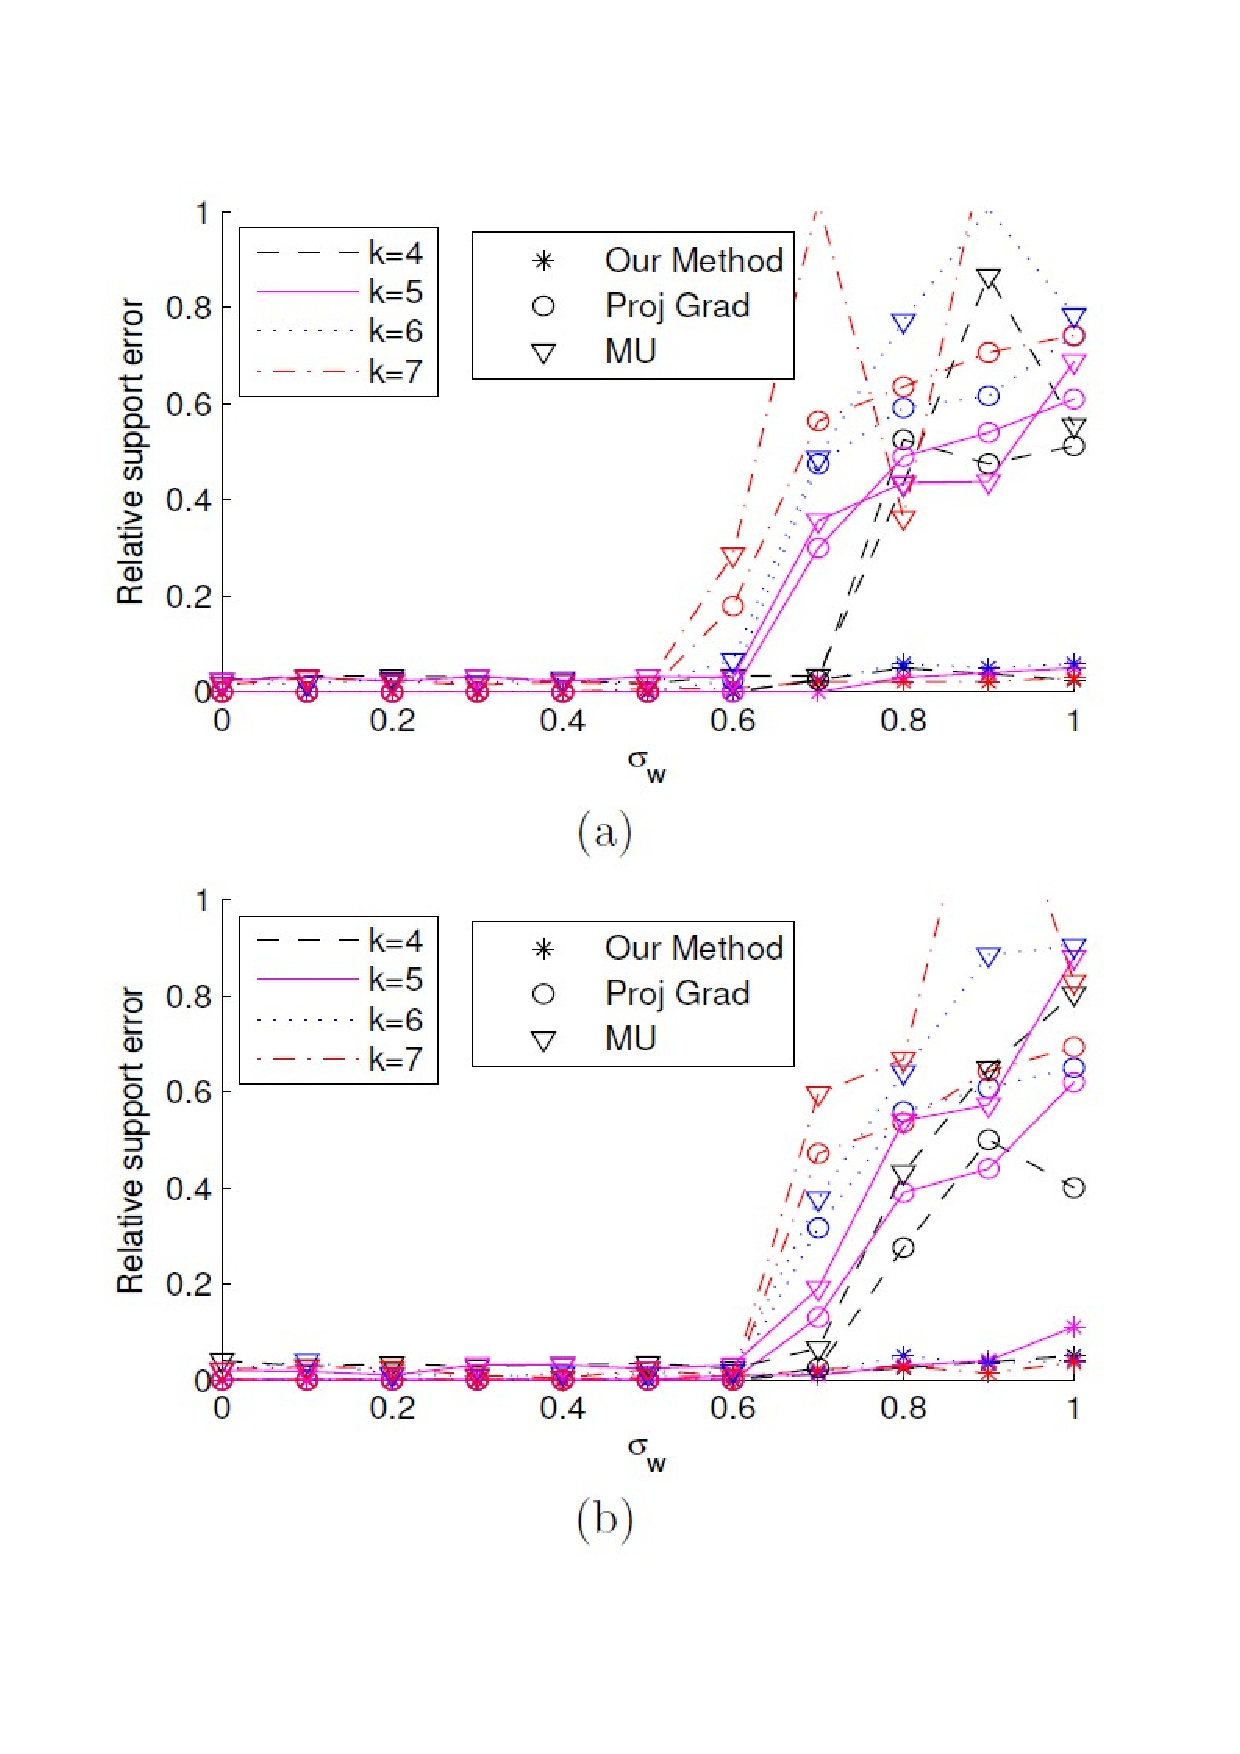
\includegraphics[scale=0.5]{relative_support_error.pdf}

\subsection{Missing Data}
We study the case with missing data, we use the following setting:\\
$p=750, n=500, \sigma_e = 0, \Sigma_w = I, k\in \{2,...,7\}$, and $\rho \in [0,0.5]$.\\
The data X and e are generated from (isotropic) Gaussian distribution. The results are shown in the graph below in which supp-OMP has better performance than other alternatives. There we have a comparison of the $l^2$ recovery error of our method. The error is plotted against the control parameter $k\frac{\sqrt{\rho}}{(1-\rho)}$.\\
(a) X has independent columns and (b) X has correlated columns.

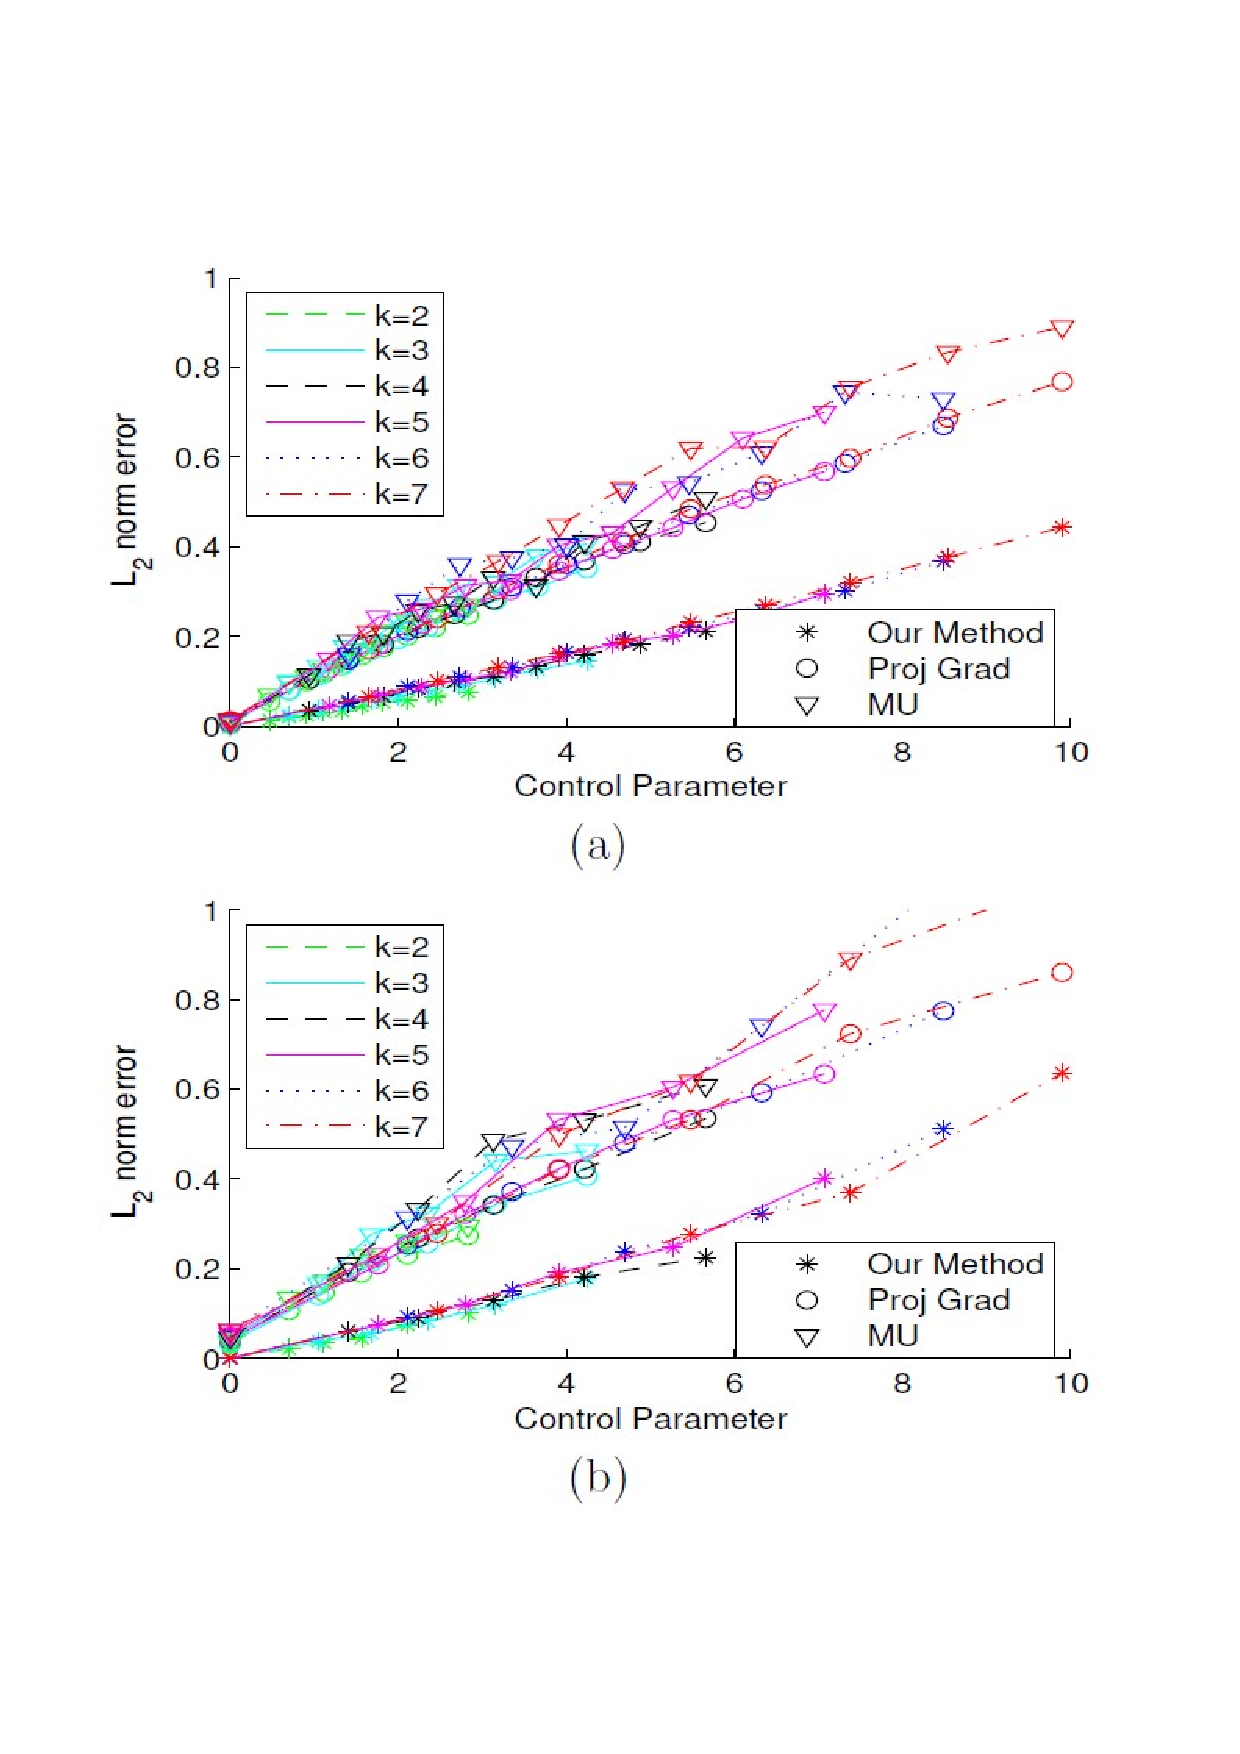
\includegraphics[scale=0.5]{l1_norm_error.pdf}


\end{document}
